\documentclass{standalone}
\usepackage{tikz}
\usepackage{ctex,siunitx}
\usepackage{tkz-euclide}
\usepackage{amsmath}
\usetikzlibrary{patterns, calc}
\usetikzlibrary {decorations.pathmorphing, decorations.pathreplacing, decorations.shapes,}
\begin{document}
\small
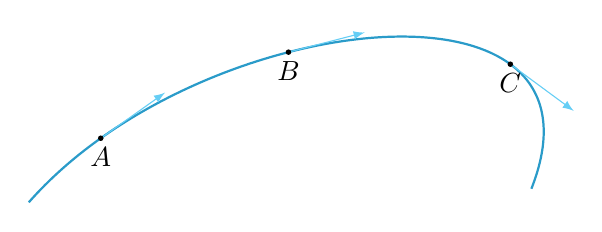
\begin{tikzpicture}[>=latex,scale=1.0]
  % \useasboundingbox(-1,-2)rectangle(8,6);
  \draw[cyan!80!black,thick](-3.798,0.497)..controls(-3.534,0.797)and(-3.224,1.069)..
  (-2.884,1.311)..controls(-2.167,1.820)and(-1.318,2.194)..
  (-0.500,2.404)..controls( 0.652,2.701)and( 1.742,2.675)..
  ( 2.318,2.251)..controls( 2.736,1.943)and( 2.883,1.425)..( 2.585,0.669);
  \draw[->,cyan!60!white](-2.884,1.311)--(-2.068,1.890);
  \draw[->,cyan!60!white](-0.500,2.404)--(0.468,2.654);
  \draw[->,cyan!60!white]( 2.318,2.251)--(3.123,1.658);
  \fill(-2.884,1.311)circle(1pt)node[below]{$A$};
  \fill(-0.500,2.404)circle(1pt)node[below]{$B$};
  \fill( 2.318,2.251)circle(1pt)node[below]{$C$};
\end{tikzpicture}
\end{document}